\let\negmedspace\undefined
\let\negthickspace\undefined
\documentclass[12pt, a4paper]{article}
\usepackage{geometry}
 \geometry{
 left=10mm,
 top=10mm,
 }
 \pagenumbering{gobble}
 \usepackage[utf8]{inputenc}
 \usepackage{graphicx}
 \usepackage{amsmath}
 \usepackage{amsfonts}
 \usepackage{amssymb}
 \usepackage{enumitem}
\usepackage{mathtools}
\usepackage[breaklinks=false]{hyperref}
\usepackage{listings}
\usepackage{calc}
\newcommand{\solution}{\noindent \textbf{Solution: }}
\newcommand{\question}{\noindent \textbf{Question: }}
\begin{document}
\title{Assignment 1}
\author{Vishal Vijay Devadiga (CS21BTECH11061)}
% make the title area
\maketitle
\question
\begin{enumerate}[label=]
\item A(-1, 3), B(4,2) and C(3,-2) are the vertices of a triangle.
\begin{enumerate}
    \item Find the coordinates of the centroid G of the triangle
    \item Find the equation of the line through G and parallel to AC.
\end{enumerate}
\end{enumerate}
\solution
\begin{enumerate}
	\begin{figure}[htbp]
	\centerline{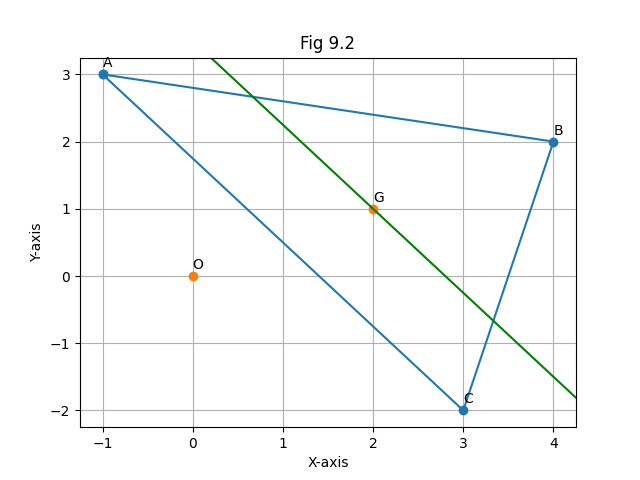
\includegraphics[scale = 1.0]{./figs/9.2.png}}
	\label{Figure 9.2}
	\end{figure}
\item Using centroid formula,
    the desired point G is given by:
    \begin{align*}
        G&= \frac{A + B + C}{3}
        \\
        &= \frac{1}{3}\{(-1,3)+(4,2)+(3,-2)\}
        \\
        &=\frac{1}{3}(6,3)
        \\
        &=(2,1)
    \end{align*}
\item Let L be the line that passes through G such that $L \parallel AC$
    Then, slope of L is equal to slope of AC.
    \begin{align*}
        m&= \frac{y_C - y_A}{x_C - x_A}
        \\
        &= \frac{-2 - 3}{3 - (-1)}
        \\
        &=\frac{-5}{4}
    \end{align*}
    G satisfies the line.
    \begin{align*}
        y_G&= mx_G + c
        \\
        c&= y_G - mx_G
        \\
        &= 1 - \frac{(-5)}{4} \times 2
        \\
        &= 1 + \frac{5}{2}
        \\
        &= \frac{7}{2}
    \end{align*}
    Thus, line L is $y = \frac{-5}{4}x + \frac{7}{2}$
\end{enumerate}
\end{document}